\documentclass[a4paper]{scrreprt}

%% Language and font encodings
\usepackage[polish]{babel}
\usepackage[T1]{fontenc}

%% Sets page size and margins
\usepackage[a4paper,top=3cm,bottom=2cm,left=3cm,right=3cm,marginparwidth=1.75cm]{geometry}

%% Useful packages
\usepackage{amsmath}
\usepackage{graphicx}
\usepackage[colorinlistoftodos]{todonotes}
\usepackage[colorlinks=true, allcolors=blue]{hyperref}

\def \GameTiTle{Technokracja}
%Technokracja

\title{\GameTiTle{}}
\subtitle{}
\author{Laura Stasiulewicz}

\titlehead{\centering
\includegraphics[width=6cm]{test.jpg}}

\begin{document}
\maketitle

\begin{abstract}
\GameTiTle{} to gra strategiczna czasu rzeczywistego. Celem gracza jest pokonanie komputerowego przeciwnika w walce o kontrolę nad punktem dominacji na mapie. Aby to uczynić, musi wykorzystać zdolność planowania, zarządzania zarówno jednostkami, jak i zasobami oraz wiedzy na temat dostępnych rodzajów oddziałów jakie może przywołać i interakcji między nimi.  %Gracz wciela się w jedną z kilku frakcji kosmicznych osadników z Ziemi walczących między sobą o kontrolę nad odległą egzoplanetą. Ze względu na słabe pole magnetyczne, nieustającą wojnę oraz odległość od innych zamieszkałych ciał niebieski ich nowy świat stał się cmentarzyskiem, a główną ucieczka z niego ambicją jego mieszkańców. 
%Short abstract of the game (max 150 words) 

\end{abstract}

{
  \hypersetup{linkcolor=black}
  \tableofcontents
}

% ______________________
% chapter Overview
% ______________________
\chapter{Przegląd}
\GameTiTle{} to gra strategiczna czasu rzeczywistego. Akcja gry umiejscowiona jest w dalekiej przyszłości, w której kolonizacja kosmosu przez ludzi jest w zaawansowanym stopniu. Koloniści docierają na odległe planety od ziemi o dekady świetlne i na nich budują nowy dom. "Nowe światy" nie są jednak dla ludzkości rajem obiecanym, osadnicy szybko dzielą się na frakcje, między którymi dochodzi do nigdy niekończących się konfliktów. Gracz wciela się w przywódcę jednego z podobnych ugrupowań walczących o kontrolę nad odległą egzoplanetą. Ze względu na słabe pole magnetyczne, nieustającą wojnę oraz odległość od innych zamieszkałych ciał niebieski ich nowy świat stał się cmentarzyskiem, a główną ucieczką z niego ambicją jego mieszkańców.
\section{Główny Zamysł}
Zamysł gry opiera się na klasycznej formule gier RTS \emph{(Real Time Strategy - ang. strategii czasu rzeczywistego)}. Ekran gry podzielony jest na mapę oraz nakładkę stanowiącej interfejs gracza. Gracz wydaje polecenia przy użyciu myszy oraz przy użyciu skrótów klawiaturowych. Rozgrywka polega na budowaniu budynków, pracowników oraz oddziałów. Budynki dzielą się na kilka rodzajów służących do zdobywania zasobów, budowania oddziałów, oraz obrony przed wrogimi oddziałami. Odziały to militarne jednostki, służące do niszczenia wrogich oddziałów, budynków oraz przejmowania punktów kontrolnych na mapie. Przeciwnikiem gracza jest sztuczna inteligencja, próbujące zrealizować identyczne cele co gracz.

\section{Co odróżnia \GameTiTle?}
W ciągu ostatnich lat gry strategiczne podzieliły się na dwa rodzaje: skupiające się na rywalizacji rankingowej między ludzkimi przeciwnikami w rozgrywkach sieciowych, wymagające dużo czasu, zaangażowania, czy energii od graczy oraz ich kompletne przeciwieństwa - gry ekonomiczne z powolnym postępem oraz kompletnym brakiem lub mocno okrojoną warstwą militarną.
\GameTiTle{} ma być powrotem do korzeni, ma nawiązywać do pierwszych serii gier RTS, gdzie głównym elementem były potyczki z komputerowymi graczami oraz scenariusze do rozgrywania przez jednego gracza. Dzięki temu osoby które lubią formułę gier tego rodzaju ale brak im czasu aby osiągnąć, często wysoki, próg umiejętności do gry sieciowej mogły także się nią cieszyć. 
W \GameTiTle{} warstwa ekonomiczna ma być nie tylko równie ważna, ale również równie rozbudowana co warstwa zarządzania jednostkami.była równie rozbudowana co militarna.

% ______________________
% chapter References
% ______________________

\chapter{Odniesienia i inspiracje} 

\section{Seria \emph{Twierdza}}
Seria \emph{Twierdza} jest bezpośrednią 
inspiracją \GameTiTle{}. Podczas gdy ekonomia wielu gier w jej gatunku sprowadza się do postawienia budynku na źródle zasobu lub wysłaniu pracownika, który ma dany zasób zbierać, w serii Twierdza twórcy zaimplementowali proste łańcuchy dostaw i przetwarzania surowców, co nadaje rozgrywce dodatkowej głębi. Ponadto widok krzątających się postaci nadaje grze niepowtarzalnego klimatu oraz imersji. \GameTiTle{} pragnie wzbogacić te elementy dodająć kompetnetnego przeciwnika SI oraz wzbogacić grę o nowoczesne elementy interfejsu, sterowania oraz silnik pozwalający na lepszą fizykę obiektów w świecie gry.

\begin{figure}[hb]
\centering
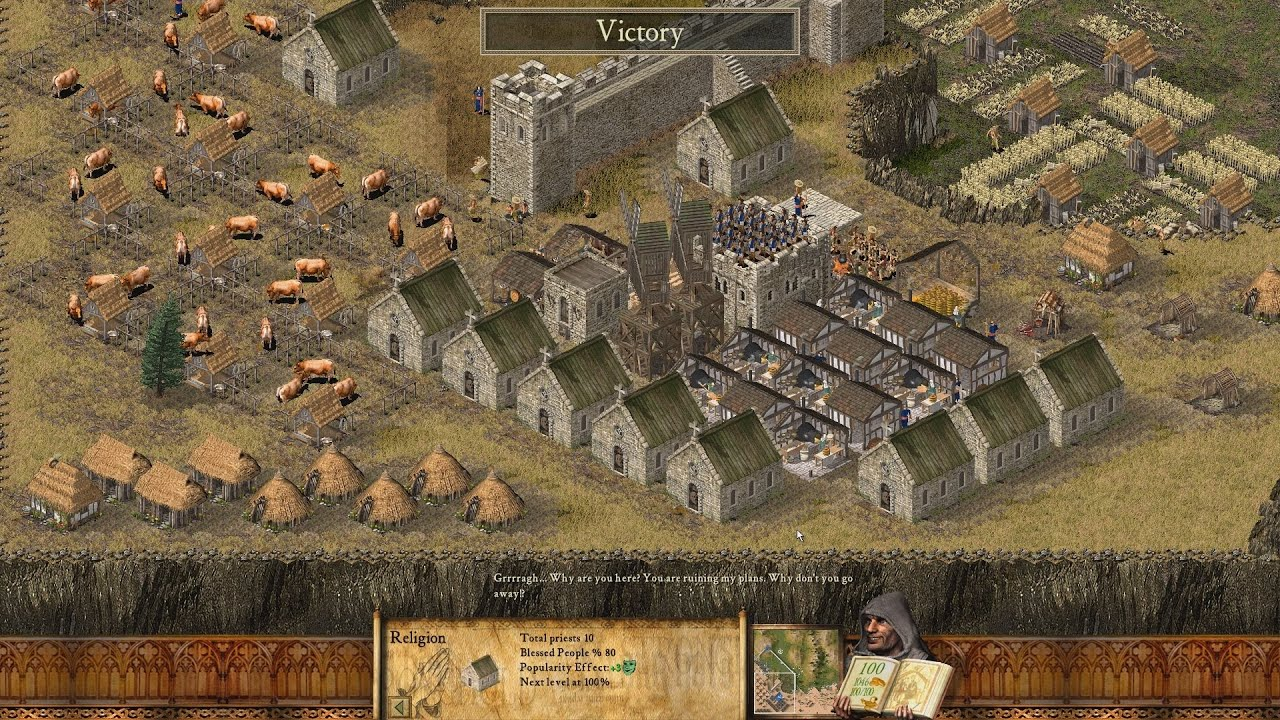
\includegraphics[width=1\textwidth]{stronghold2.jpg}
\caption{\label{} Zrzut ekranu z gry Twierdza}
\end{figure}
\newpage

\section{Seria \emph{Company of Heroes}}
Seria \emph{Company of Heroes} odznaczyła się nie tylko poprzez doskonale rozwinięty tryb sieciowy, ale także poprzez dużo ilość zawartości dla pojedynczego gracza oraz za ikoniczny tryb walki nad sektorami zwycięstwa. Ważnym elementem rozgrywki była doktryna sił połączonych: gracz musiał umiejętnie dopierać kompozycję swojej armii, aby móc odpowiadać na ataki przeciwnika. 
W \GameTiTle{} te elementy wprowadzimy na własny sposób, łącząc taktyczne aspekty serii z bardziej rozbudowaną warstwą ekonomiczną.

\begin{figure}[hb]
    \centering
    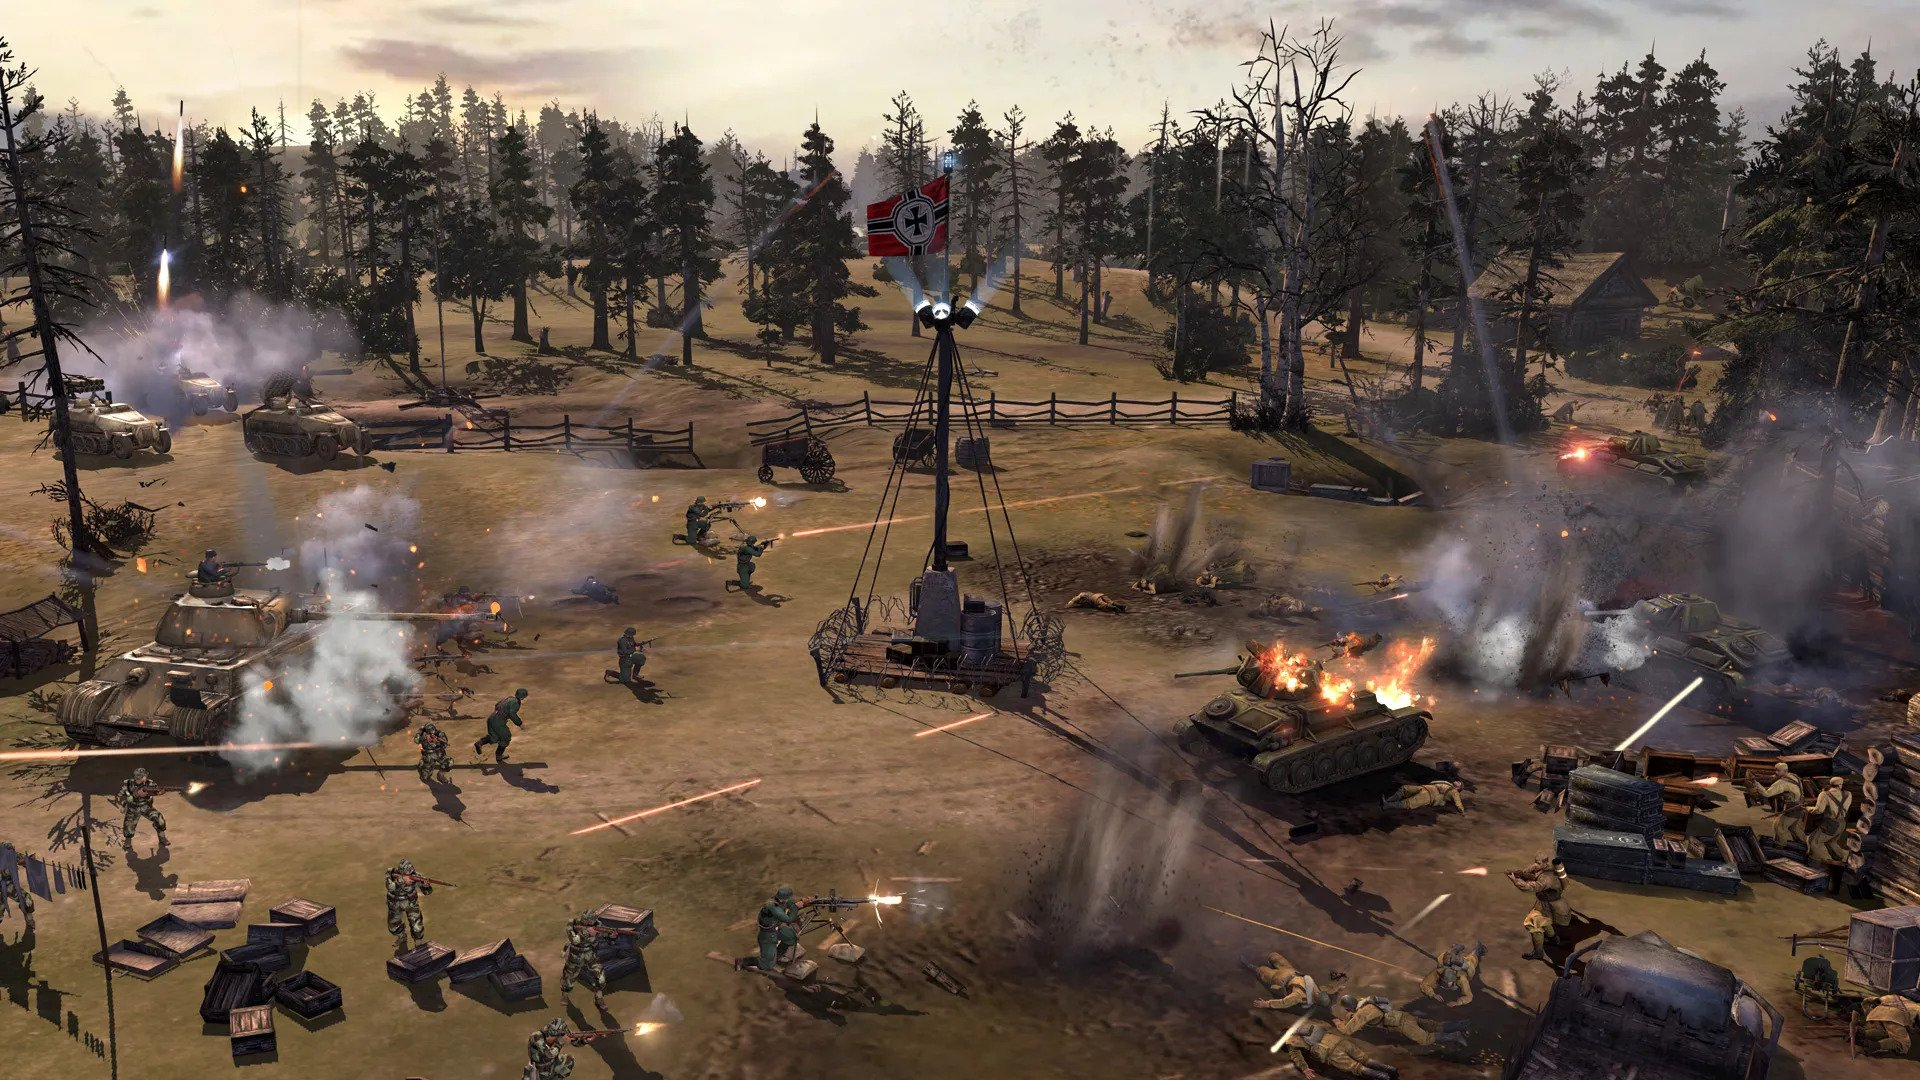
\includegraphics[width=1\textwidth]{coh2.jpg}
    \caption{\label{} Walka o sektor kontrolny w grze Company of Heroes 2}
    \end{figure}

% ______________________
% chapter Specification and Market Analysis 
% ______________________

\chapter{Szczegóły techniczne}
%description of target group, platform, art style, who to attract of how to attract 

\section{Grupa docelowa}
Osoby po 18 roku życia, fani klasycznych strategii, osoby, które spędzają średnio od 3 do 12 godzin tygodniowo na graniu w gry komputerowe.

\section{Gatunek}
Gra należy do gatunku strategii czasu rzeczywistego.
\section{Styl graficzny}
Gra będzie wykorzystywać grafikę 2D, z wykorzystaniem techniki \emph{Pixel Art.}

\begin{figure}[hb]
\centering
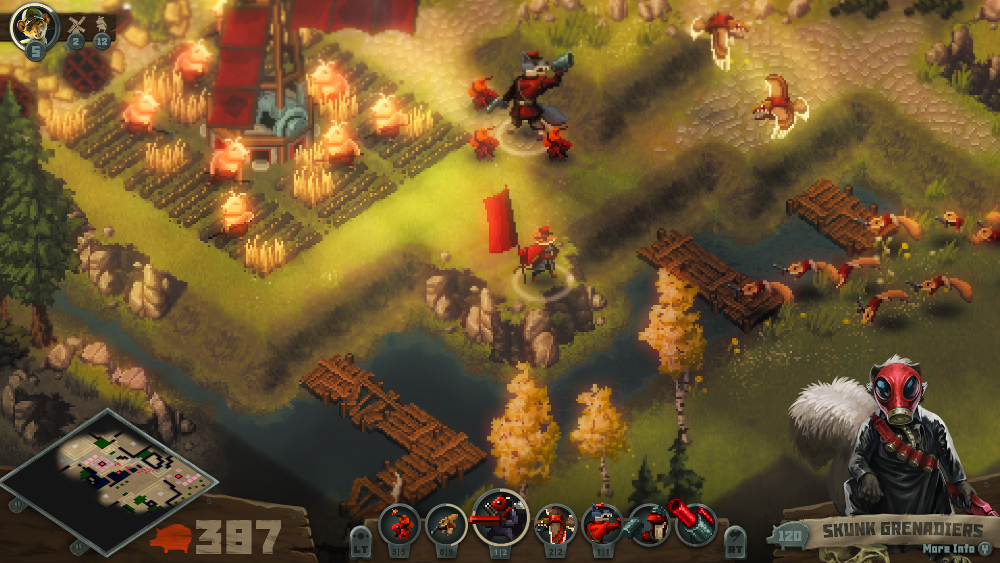
\includegraphics[width=1\textwidth]{ToothAndTail.png}
\caption{\label{fig:arteg1} Przykład grafiki w stylu Pixel Art (Tooth and Tail, Pocketwatch Games)}
\end{figure}

\begin{figure}[hb]
  \centering
  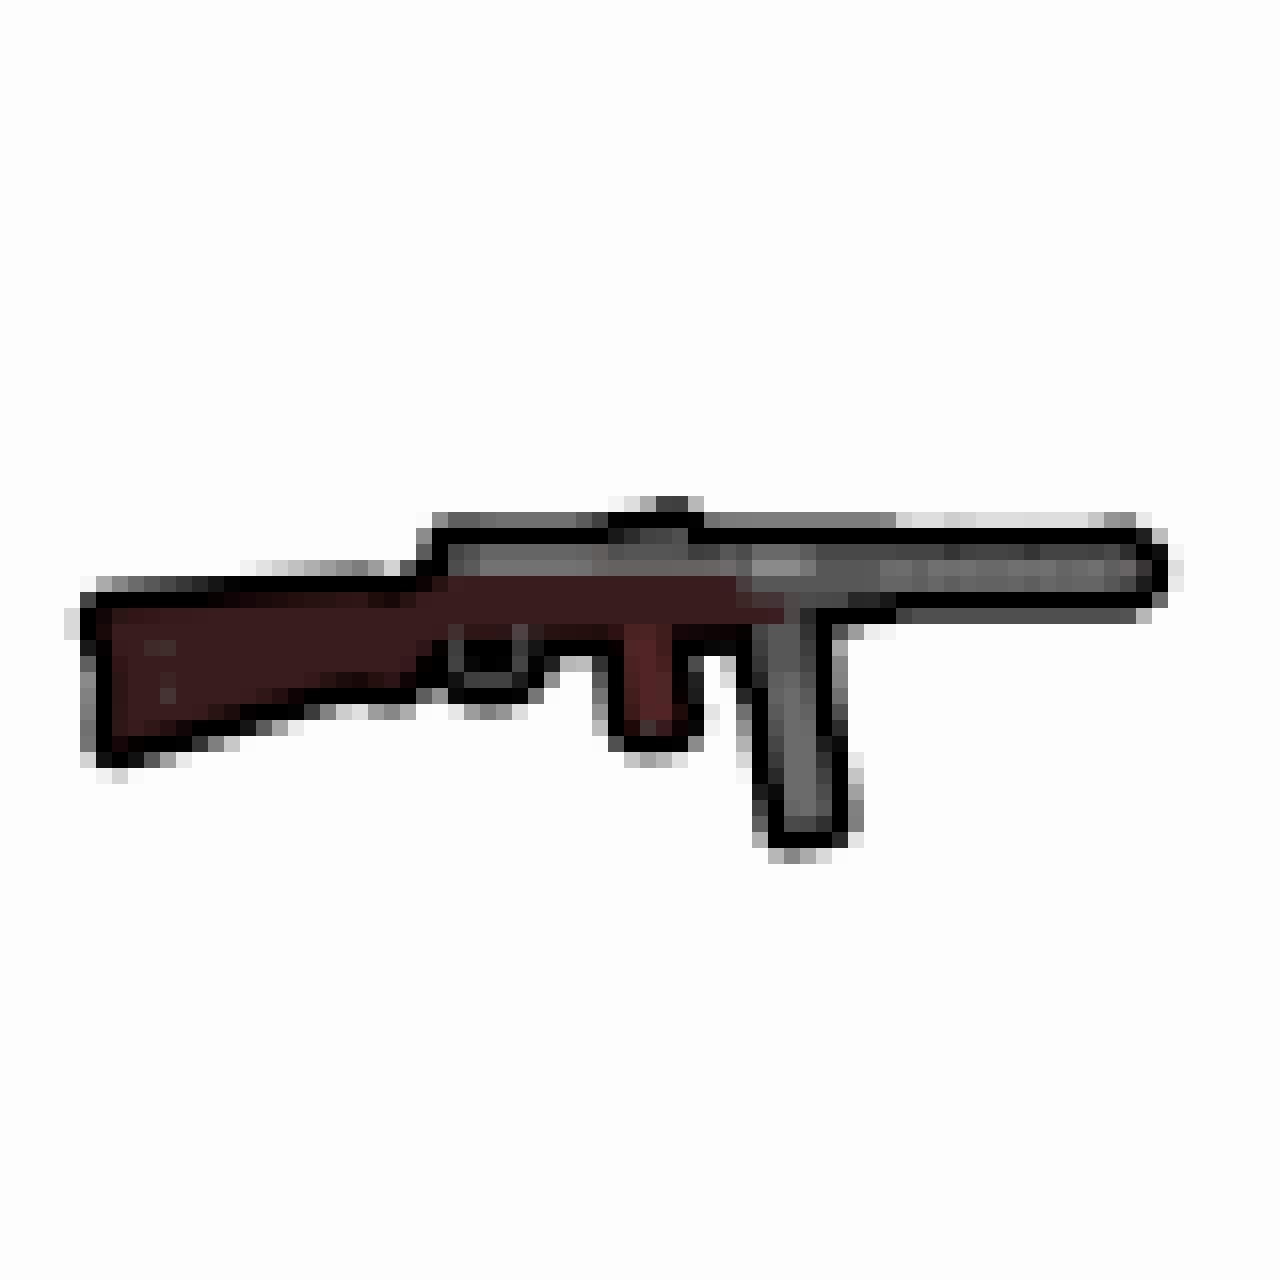
\includegraphics[width=0.6\textwidth]{morswpng.png}
  \caption{\label{fig:arteg2} Przykład grafiki wykonanej w stylu Pixel Art}
  \end{figure}


\section{Formy Zaangażowania Gracza}
%thinking of Hunicke's 8 kinds of "fun" - what would you like to focus on?\\
% (1. Sensation - Game as sense-pleasure 
% 2. Fantasy - Game as make-believe
% 3. Narrative - Game as drama
% 4. Challenge - Game as obstacle course
% 5. Fellowship -  Game as social framework
% 6. Discovery - Game as uncharted territory 
% 7. Expression - Game as self-discovery 
% 8. Submission - Game as pastime)
\GameTiTle{} pozwala graczowi sprawdzić się w wyzwaniu, jakim będzie pokonanie przeciwnika SI. Będzie musiał to tego wykorzystać zarówno zręczność, jak i umiejętność strategicznego myślenia. Oprócz tego gra oferuje wczucie się w rolę uczestnika 

% ______________________
% chapter Game Details
% ______________________


\chapter{Gameplay and Game Setting}
be specific about the core game features 

\section{Mood and Emotions}
what mood and emotions does the game create (can change e.g. for every level / section) 

\section{Story}
the story of the game

\section{World/Environment}
what is the settings of the game 

also, add here a map of your environment or a picture of your world if necessary

\section{Objects in the Game}
what objects will be in the game?

\section{Characters in the Game}
who are the characters in the game?

\section{Main Objective}
what is the goal / main objective of the game?

\section{Core Mechanics}
very important section: what are the core mechanics? be specific

\section{Controls}
describe the controls of the game 
also, add here a controller diagram if necessary 

% ______________________
% chapter Front End
% ______________________


\chapter{Front End}
description of front end such as start screen, menu screens,..  

\section{Start Screen}

\section{Menus}

\section{End Screen}

% ______________________
% chapter Game Details
% ______________________


\chapter{Technology}
what technologies is the game designed for, what is the target platform, what technologies are used for the development? 

\section{Target Systems}
what platforms is the game designed for

\section{Hardware}
what hardware is needed to play the game? any additional interface? recommended controllers? 

\section{Development Systems/Tools}
please describe the tools you are using (game engine, art tools, ..) 

% ______________________
% chapter Game Details
% ______________________


\chapter{Topic and Inclusion }

describe here how you plan to address the main topic (main theme) and topics around inclusion

\section{Main Theme}
\section{Inclusion}

\subsection{Diversity}
diversity in games is an important topic. please describe here how you addresses diversity in your game and game design elements 
\subsection{Accessibility}
make your games more accessible. use this section to describe what guidelines you addresses and how you cater for  gamers with disabilities and other impairments. great reference: \url{http://gameaccessibilityguidelines.com/}
%\subsection{Humanity}

% ______________________
% chapter Game Details
% ______________________


\chapter{Timeline and Cost Estimation}

In this chapter, you should describe your planned time management, the estimation of how long you think your team will need and how much you think this project would cost. 

Tools we recommend for project management are for instance \url{https://app.hacknplan.com/login}. To track your time, we recommend \url{https://toggl.com/}.  

\begin{table}[h]
\centering
\begin{tabular}{|l|l|l|}
\hline
Milestone & Description & Date \\\hline
& Official Start Date & 01.12.... \\
1 & Milestone Description ..  & 01.12.... \\
2 & Milestone Description ..  & 01.01.... \\
3 & Milestone Description ..  & 01.03.... \\
& End of Project & 01.04.... \\
\hline
\end{tabular}
\caption{\label{tab:schedule}Example Schedule.}
\end{table}

\section{Time Estimation}

While working on your project you should track your time. 
We recommend using \url{https://toggl.com/} for time management. In the final report you will have to compare the estimated time with the actual time. (Miscalculation do not have any effect on your grade!!!)

\section{Cost Estimation}

Estimated cost of the project based the described tasks and milestones and the  time estimation.  

% ______________________
% chapter Game Details
% ______________________


\chapter{Team and Credits}

most important - who are you, who takes what role? 

e.g. :
Project Management: \\
Programming: \\ 
Art: \\ 
Design: \\ 

Additional Credits (e.g. sources of art, audio,.. ) 

%\todo[inline, color=green!40]{This is an inline comment.}

%\bibliographystyle{alpha}
%\bibliography{sample}

\end{document}